
% Licensed to the Apache Software Foundation (ASF) under one or more
% contributor license agreements. See the NOTICE file distributed with
% this work for additional information regarding copyright ownership.
% The ASF licenses this file to You under the Apache License, Version 2.0
% (the "License"); you may not use this file except in compliance with
% the License. You may obtain a copy of the License at
%
%     http://www.apache.org/licenses/LICENSE-2.0
%
% Unless required by applicable law or agreed to in writing, software
% distributed under the License is distributed on an "AS IS" BASIS,
% WITHOUT WARRANTIES OR CONDITIONS OF ANY KIND, either express or implied.
% See the License for the specific language governing permissions and
% limitations under the License.

\documentclass[letterpaper,onecolumn,12pt,titlepage]{article}
\setlength{\textheight}{9in}
\setlength{\columnsep}{0.25in}
\setlength{\textwidth}{6.5in}
\setlength{\topmargin}{0in}
\setlength{\headheight}{0in}
\setlength{\headsep}{0in}
\evensidemargin=0in
\oddsidemargin=0in
\usepackage{amsmath}
\usepackage{amssymb}
\usepackage[pdftex]{graphicx}
\usepackage{subfigure}
\usepackage[T1]{fontenc}
\title{Apache Accumulo Developer's Manual - Version 1.3}
\author{}
\begin{document}
\maketitle
\newpage
\tableofcontents
\newpage
\section{Introduction}

\begin{figure}[htbp]
\center
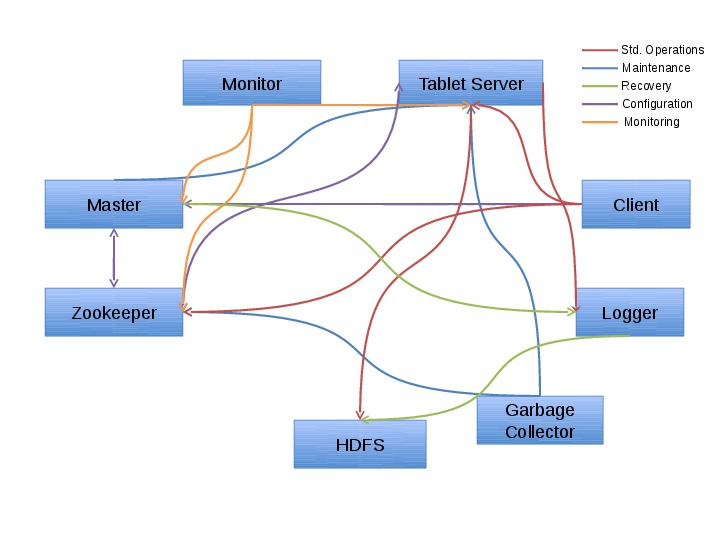
\includegraphics[scale=.6]{images/component_overview.jpg}
\caption{\label{fig_overview} Overview of Apache Accumulo components.}
\end{figure}
This manual is designed for the use of programmers who wish to understand the inner workings of Accumulo, as well as those who would like to participate in Accumulo development.
In this manual we describe the interactions between Accumulo components, and attempt to orient the reader to how and where those interactions are implemented in the source code.

Accumulo includes several components, some of which are externally developed systems.
These components and their interactions are shown at a high level in figure \ref{fig_overview}.
External components include Zookeeper, HDFS and Hadoop Map-Reduce.
Zookeeper is used as a small, highly available key/value store to host configuration information.
Zookeeper is also used as a distributed locking service with no single point of failure.
HDFS is used as the underlying file system for Accumulo, and it handles replicating data, balancing data storage across disks, and providing a consistent view from each node in the cluster.

Hadoop Map-Reduce can be used as a client of Accumulo, but we will defer to the client component for a description of that interaction.

Internal Accumulo components include the Tablet Server, the Master, the Client, the Logger, the Garbage Collector, and the Monitor.
The Tablet Server is responsible for hosting read and write activities for non-overlapping partitions of the key space in Accumulo tables, called Tablets.
The Master plays a coordinating role in the cluster, balancing Tablet load across Tablet Servers, and servicing a number of infrequent configuration requests like table creation and user management.
The Client in this documentation refers to the set of Java classes that interface between user code and these Accumulo components.
The Logger is responsible for streaming write-ahead logs to disk, and also plays a role alongside the Master, HDFS and the Tablet Server in recovering a failed Tablet.
The Garbage Collector performs a reference counting operation to clean up data files and write-ahead logs that are no longer referenced in Tablet Metadata.
The Monitor collects statistics about existing tables, operations, warnings, and errors, and makes that information available via a web service.
Each of the aforementioned internal components is described by a series of illustrations in this documentation, and its interactions are viewed from the perspectives of read/write operations, maintenance, recovery, configuration, and monitoring.

\section{Tablet Server}

\subsection{Read/Write Operations}
\begin{figure}[htbp]
\center
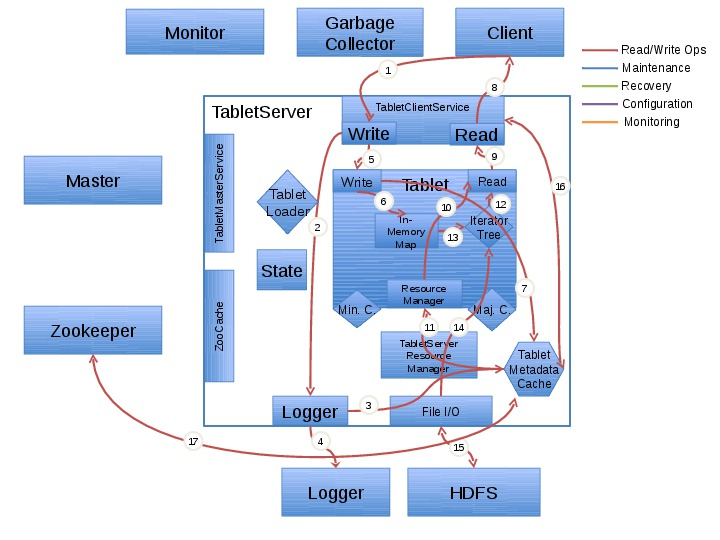
\includegraphics[scale=.6]{images/tserver_rw.jpg}
\caption{\label{fig_ts_rw} Tablet Server read/write operations.}
\end{figure}

% introduce read/write operations
Figure \ref{fig_ts_rw} shows the Tablet Server data flow during regular read/write operations.
All of the descriptions in this section will refer to the data flows shown in figure \ref{fig_ts_rw}.
In (1) and (8), the Client contacts RPCs within the Thrift service hosted on the TabletServer. 
These RPCs are all the org.apache.accumulo.server.tabletserver.TabletServer.ThriftClientHandler, that implements the org.apache.accumulo.core.tabletserver.thrift.ThriftClientHandler.Iface interface.
Methods within this interface are divided into read and write methods.

% introduce write RPCs
The write methods used by (1) are split into three sets of RPC calls: single updates, sessionized writes (for batch writes) and bulk updates.
These calls result in further calls throughout the Tablet Server, as shown in (2) through (7).

% discuss single update RPC
Single update calls use the synchronous update(AuthInfo, KeyExtent, Mutation) method, which only returns when the given Mutation has been applied.
The update(AuthInfo, KeyExtent, Mutation) method checks the given AuthInfo against the set of users allowed to write to the given Tablet, 
looks up the specified Tablet in the list of online Tablets, logs the Mutation to the write-ahead log as seen in (2) through (4) and described below, 
and then sends the given Mutation to the commit(int, List$<$Mutation$>$) method of the Tablet as operations (5) and (6), also described below.
If any of these parts fails, an exception is thrown to the client.

Sessionized updates use the startUpdate(AuthInfo), setUpdateTablet(long, KeyExtent), applyUpdate(long, Mutation), and closeUpdate(long) methods.
startUpdate(AuthInfo) is a synchronous RPC that checks the authorization info, creates a session, and then passes back a secure, random, long session ID that is used by the client to refer to this session for all other RPC methods.
Once a session is created, the client will select a tablet to mutate using the asynchronous setUpdataTablet(long, KeyExtent) method and can change that tablet as often as desired.
After selecting a tablet the client can send mutations using the asynchronous applyUpdate(long, Mutation) method zero or more times per tablet.
At the end of the session the client calls the synchronous closeUpdate(long) method, which only returns when the entire session has been committed.
closeUpdate(long) returns the list of tablets that had errors, and how many mutations were successfully applied to those tablets, as well as a summary of the constraint violations and authorization failures that occurred in the given session.

% describe logging procedure (steps 2-4)

When mutations arrive at the tablet server (1), they are cached briefly to queue up many streamed mutations for the same session.
If cache memory fills, or a session is closed, the Mutations are flushed (2) through to a local Logger component which 
forwards the updates to a remote Logger service (4) using a RPC interface. 
In order to provide redundancy, the mutations are sent to two different Logger servers in the cluster.
The Tablet Server records what logs are used (3) by each tablet in the Metadata Table describing the tablet.
When a Tablet Server fails, its Tablets are reassigned by the Master, 
and the surviving Tablet servers can replay lost Mutations from the logs listed in the Metadata table.


% describe tablet write procedure (steps 5-6)
Operation (5) represents the interaction between the TabletServer ThriftClientHandler and the commit(int, List$<$Mutation$>$) method within the org.apache.accumulo.server.tabletserver.Tablet class.
This method is called by the single update and batch update API calls.
Within the commit method, each Mutation is expanded to a set of key/value pairs, all of which are added to the in-memory map as an atomic operation, operation (6).
The in-memory map could be implemented as either a TreeMap of Text to TreeMaps or a native C++ Map of byte arrays to Maps, each of which maps rows to maps of columns to values.

% describe bulk ingest
The third mechanism for writing data to Accumulo is known as bulk ingest, during which whole map files are added to a table instead of individual Mutations.
For bulk ingest the client calls the bulkImport(AuthInfo, Map$<$KeyExtent, Map$<$String, MapFileInfo$>$$>$) method.
This method directly adds a set of map files for each Tablet named by the given KeyExtent objects.
For each given KeyExtent, bulkImport looks up the tablet that the KeyExtent describes in the set of online tablets and passes it the map of filenames (String) to file stats (MapFileInfo) via its importMapFile(Map$<$String,MapFileInfo$>$) method.
This method directly adds the given files to the set of active files for the given tablet as shown in (7).
Bulk ingest bypasses the logging mechanism and in-memory map completely (operations (2) through (6)), so it can be very efficient if the map files can be easily produced outside of Accumulo.

Read RPCs used in (8) are split into TODO ...

\subsection{Maintenance}
\begin{figure}[htbp]
\center
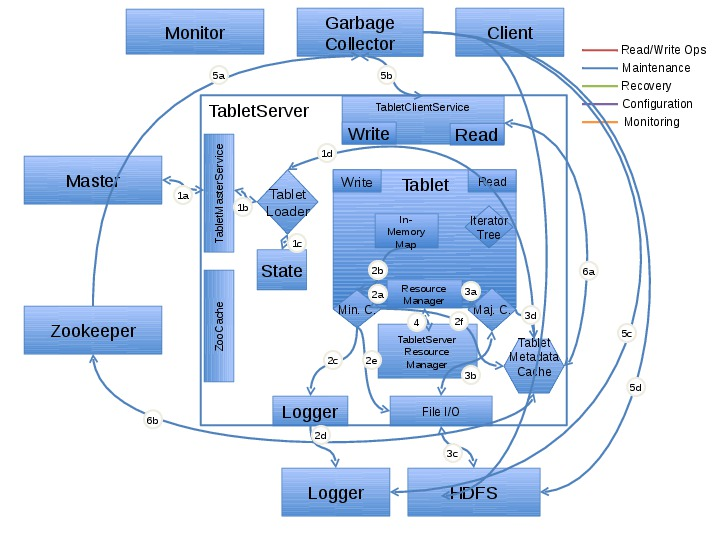
\includegraphics[scale=.6]{images/tserver_maintenance.jpg}
\caption{\label{fig_ts_maintenance} Tablet Server maintenance operations.}
\end{figure}

Maintenance operations from the perspective of the Tablet Server fall into several categories: loading, unloading, and migration of Tablets; Tablet Server status monitoring; minor compactions; major compactions; splits; and garbage collection of RFiles and write-ahead logs.

Tablet loading, unloading, and migration operations are all initiated by the Master as calls to the loadTablet and unloadTablet functions of the TabletClientService.IFace Thrift interface, which is hosted on the Tablet Server as an instance of TabletServer.ThriftClientHandler.
Load and unload operations execute in the background as tasks that are performed by Executors located in the TabletServerResourceManager.
% TODO discuss how load and unload execute

Tablet Server status monitoring is initiated by the Master via a call to the getTabletServerStatus method of TabletClientService.

% TODO: discuss minor compactions
% TODO: discuss major compactions
% TODO: discuss splits
% TODO: discuss garbage collection

\subsection{Recovery}
\begin{figure}[htbp]
\center
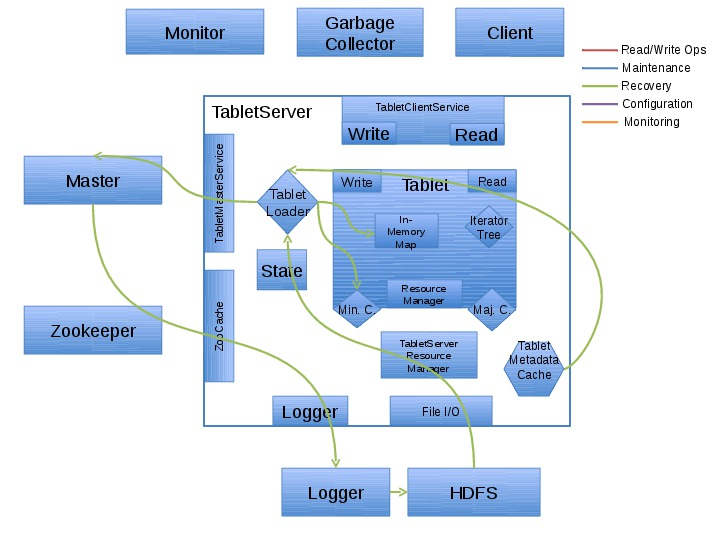
\includegraphics[scale=.6]{images/tserver_recovery.jpg}
\caption{\label{fig_ts_recovery} Tablet Server recovery operations.}
\end{figure}

\subsection{Configuration}
\begin{figure}[htbp]
\center
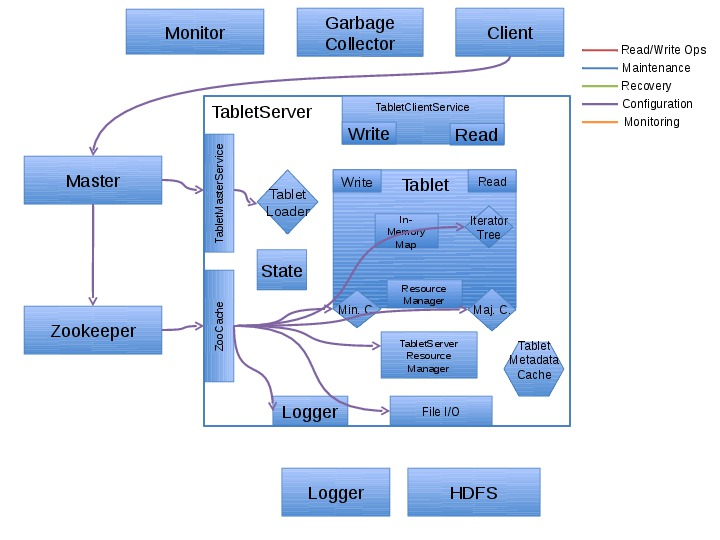
\includegraphics[scale=.6]{images/tserver_config.jpg}
\caption{\label{fig_ts_config} Tablet Server configuration operations.}
\end{figure}

\subsection{Monitoring}
\begin{figure}[htbp]
\center
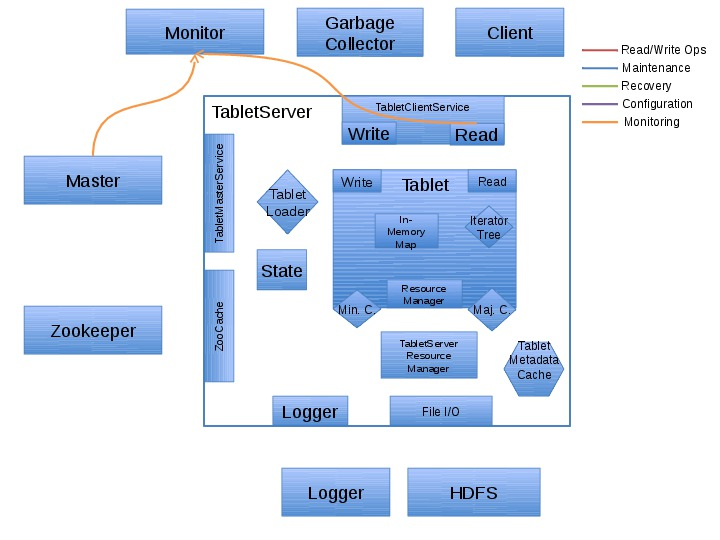
\includegraphics[scale=.6]{images/tserver_monitor.jpg}
\caption{\label{fig_ts_monitor} Tablet Server monitoring operations.}
\end{figure}

\section{Master Operations}
\subsection{Load Balancer}
\subsubsection{Introduction to Accumulo Load Balancers}

In Accumulo 1.3, a load balancer recommends tablet assignments (in the case of unassigned tablets) and tablet migrations (moves from one server to another).
The load balancer is run on the master server.
The getServerForTablet and getMigrations functions are continually polled and should be designed to be executed fast.
Load Balancers should not be designed to make any thrift calls to the master server since this can create a deadlock.
Load Balancers are Administrator selectable and programmable.
The default load balancer in Accumulo 1.3 is DefaultLoadBalancer.
DefaultLoadBalancer distributes tablets to servers so that the number of tablets on a given server is equal to the high number of tablets, ceil(total number of tablets/total number of servers), or the low number of tablets, floor(total number of tablets/total number of servers), with an equal number of tablets from each table on every server.
When a tablet splits and the tablet server hosting the tablet is equal to the low number of tablets, the tablet stays where it is and does not migrate to another server.
When a tablet splits and it is on a tablet server with the high number of tablets, the tablet is migrated to the first server with the low number of tablets.
Introduced in Accumulo 1.2 are table load balancers.
These load balancers are responsible for load balancing a particular table of the cluster.
They can be specified using the table property table.balancer.
To use a table load balancer, the cluster must be running TableLoadBalancer as the system wide load balancer.
This load balancer takes care of the details of grouping the tablets up by table and sending load balancing information to the appropriate table load balancers.
This load balancer will by default, load the simple load balancer for every table.
Creating a load balancer requires writing your own implementation in Java that implements the TabletBalancer interface.


\section{Client Library}
\section{Logger Operations}
\section{Garbage Collector Operations}

\end{document}
